\documentclass[tikz,border=2pt,11pt]{standalone}
\usetikzlibrary{arrows.meta}
\usetikzlibrary{calc}
\usepackage{amsmath}
\usepackage{amssymb}
\usepackage{graphicx}
\usepackage{tikz}
\newcommand{\R}{\mathbb R}
\DeclareMathOperator{\crn}{cr}
\DeclareMathOperator{\rank}{rank}
\DeclareMathOperator{\Span}{span}
\DeclareMathOperator{\diag}{diag}
\begin{document}
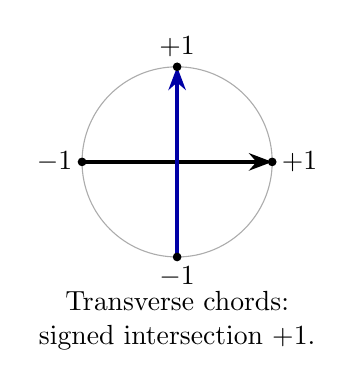
\begin{tikzpicture}[scale=1.05,>=Stealth]
  \draw[gray!65] (0,0) circle (1.15);
  \draw[->,very thick] (-1.15,0)--(1.15,0);
  \draw[->,very thick,blue!65!black] (0,-1.15)--(0,1.15);
  \foreach \x/\y in {-1.15/0,1.15/0,0/-1.15,0/1.15}
    \fill (\x,\y) circle (1.5pt);
  \node[left] at (-1.15,0) {$-1$};
  \node[right] at (1.15,0) {$+1$};
  \node[below] at (0,-1.15) {$-1$};
  \node[above] at (0,1.15) {$+1$};
  \node[align=center] at (0,-1.92) {Transverse chords:\\signed intersection $+1$.};
\end{tikzpicture}
\end{document}
